Zu Beginn der Umsetzung wurde die Anbindung der neuzuschaffenden Erweiterung zur Erfassung der Daten aus dem Signatur-Tablet sowie die Weitergabe und Integration in den bestehenden Datenbestand der Sage Office Line durch FZP analysiert. Anschließend wurden verschiedene Anbieter von Signatur-Tablets geprüft. Hier hat sich die Firma Wacom schnell heraus kristallisiert, hinsichtlich der Unternehmenserfahrungen seit 1983 \cite{konzept1}. Ein weiteres positives Merkmal ist die guten Anbindung des grafischen Tablets mittels des bereit gestellten Software Developer Kits (SDK)\footnote{\label{foot:4}Software Development Kit: Sammlung von Werkzeugen und Anwendungen, um eine Software zu erstellen, meist inklusive Dokumentation. \cite{SDK}}. Nach Abschluss der Prüfungen wurde mit der Entwicklung der Erweiterung begonnen. Die Entwicklung von Zusatzmodulen und Erweiterungen ist angesichts des modularen Aufbaukonzepts der Sage Office Line möglich. Die Einbindung von Erweiterungen wird mit einer eigenentwickelten Methode von Sage, namens Dynamic Link Library\footnote{\label{foot:6}Dynamic Link Library: Dynamische Programmbibliothek für Microsoft Betriebssysteme. \cite{DLL}} (DLL) Common Method (DCM) realisiert. Mit dieser Methode können Anpassung an der Sage Office Line auf Basis des Microsoft .NET Frameworks\footnote{\label{foot:5}Framework: Grundstruktur / Rahmenwerk zur Bestimmung der 
Software-Architektur. Es besteht aus mehreren Klassen, die zusammenarbeiten und wieder verwendbare Entwürfe darstellen. \cite{framework}} vorgenommen werden. Mit Hilfe von DCM werden die Anpassungen mit der verwendeten Technologie der Sage Office Line auf Basis von Microsoft Access in Verbindung mit dem Microsoft Component Object Model Frameworks (COM) verbunden. Zuerst ist die Einbindung der benötigten DLLs in das Microsoft .NET Entwicklungsprojekt notwendig. Die DLLs umfassen unteranderen die benötigten Komponenten zur Kommunikation zwischen der Erweiterung, der Sage Office Line und dem Signatur-Tablet. Des Weiteren werden die DLLs des Signatur-Tablets zur Erfassung und Prüfung der biometrischen Unterschrift eingebunden. Das Entwicklungsprojekt ist in die Projekte "'FZP.OfficeLine.Abf.Signatur"' und "'FZP.Wacom"' unterteilt. Die Aufteilung in Unterprojekte wurde angesichts der Wiederverwendbarkeit von einzelnen Projektteilen gewählt.
\begin{figure}[!ht]
    \centering
    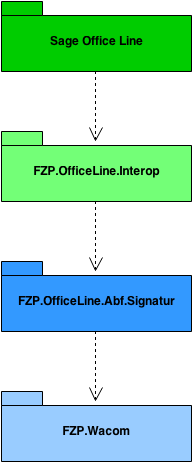
\includegraphics[height=210pt, width=100pt]{paketDiagrammNeu2.png}
    \caption[Paketdiagramm FZP.Wacom.Erweiterung]{\small{Paketdiagramm FZP.Wacom.Erweiterung}}
\end{figure}
\newline
Das in der nächsten Seite dargestellte Klassendiagramm symbolisiert das Projekt "'FZP.OfficeLine.Abf.Signatur"'. Der rot umrandete Bereich zeigt die Klassen, die die Anbindung an die Sage Office Line regeln. Es existieren zwei Klassen, welche die Erfassungsmaske für die biometrische Unterschrift aus der Sage Office Line heraus öffnen können. Die Erfassungsmaske kann im Standard des Verkaufsbereichs der Sage Office Line sowie im Zusatzmodul FZP Vermietung gestartet werden.
\begin{figure}[!ht]
    \centering
    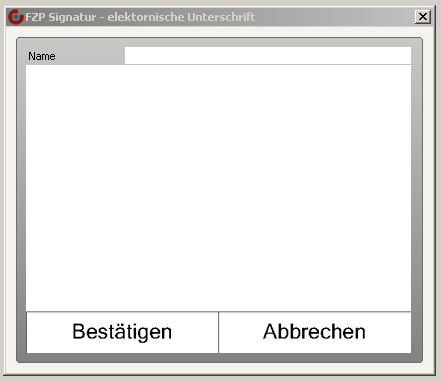
\includegraphics[height=300pt, width=300pt]{steuerelement.PNG}
    \caption[Erfassungsmaske biometrische Unterschrift]{\small{Erfassungsmaske biometrische Unterschrift}}
\end{figure}
\newline
Der blau umrandete Bereich kennzeichnet die Klasse der Erfassungsmaske. Die Erfassungsmaske enthält das geschaffene Steuerelement zur Erfassung der biometrischen Unterschrift. Weiterhin regelt die Maske den Funktionsaufruf zur Speicherung der biometrischen Unterschrift. Ebenfalls wird das Öffnen und Schließen der Erfassungsmaske gesteuert. Der grün umrandete Bereich zeigt die Klasse des Signaturbelegs. Diese dient zum Speichern, Aktualisieren und Laden von biometrischen Unterschrift. Des Weiteren erfolgt eine Prüfung, ob bereits biometrische Unterschrift für den jeweiligen Vorgang vorhanden sind. Darüber hinaus enthält der grüne Bereich eine Klasse mit Funktionen zur Prüfung der Datenbank und deren Version sowie zur Aktualisierung. Die Klasse dient zum Erstellung und Schließen einer Datenbankverbindung. Sie regelt ebenfalls die Ausgabe von Hinweis- und Fehlermeldungen.
\begin{figure}[!ht]
    \centering
    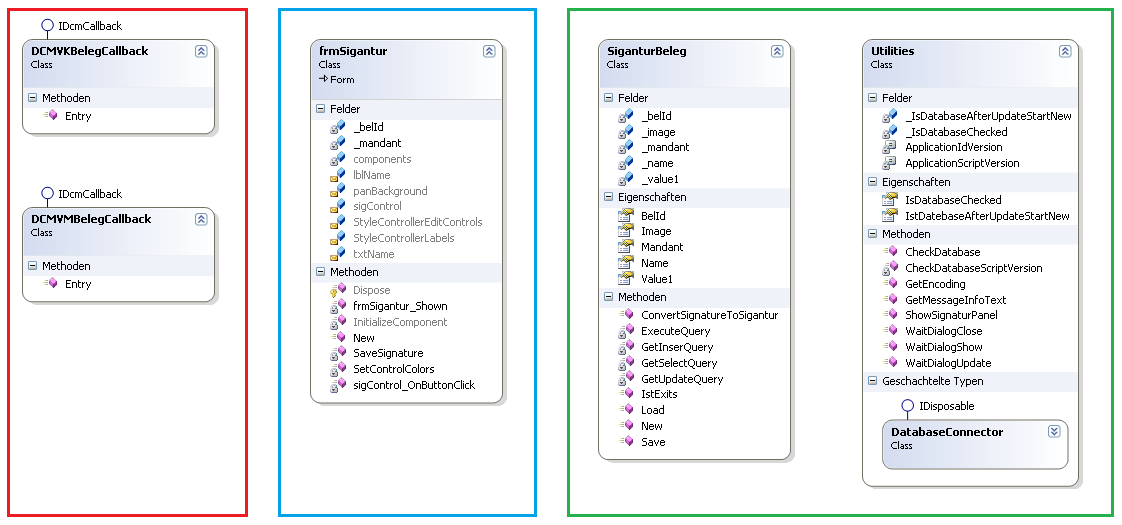
\includegraphics[height=300pt, width=\textwidth]{Klassendiagramm_Abf_Signatur_Edit2.png}
    \caption[Klassendiagramm FZP.OfficeLine.Abf.Signatur]{\small{Klassendiagramm FZP.OfficeLine.Abf.Signatur}}
\end{figure}
\newline
\pagebreak
\textbf{} %Workaround
\newline
Das Klassendiagramm auf der folgenden Seite symbolisert das Projekt "'FZP.Wacom"'. In diesem Projekt wurde im blau umrandeten Bereich das Steuerelement zur Darstellung der biometrischen Unterschrift auf einem Bildschirm geschaffen. Die Funktionen des Steuerelements sind auf der einen Seite die Ermittlung des verwendeten USB bzw. COM-Port des Computers an dem das Signatur-Tablets angeschlossen ist. Auf der anderen Seite wird die Zeichnung des Erscheinungsbilds des Steuerelements, die Entfernung des Unterschriftsbilds vom Display des Tablets und das Schließen des Steuerelements durchgeführt. Die Klassen im grün umrandeten Bereich sind für die folgenden Funktionen zuständig. Das Steuerelement reagiert auf die Eingaben des Signatur-Tablets und leitet diese an die Klassen zur Sammlung, Prüfung und Aufbereitung der Daten aus dem Signatur-Tablet weiter. Danach werden die Daten an die Eingabemaske zur Darstellung weiter geleitet. Abschließend wird mit den aufbereiteten Daten die biometrische Unterschrift erstellt und an die Klasse Signaturbeleg zur Speicherung übergeben.
\begin{figure}[!ht]
    \centering
    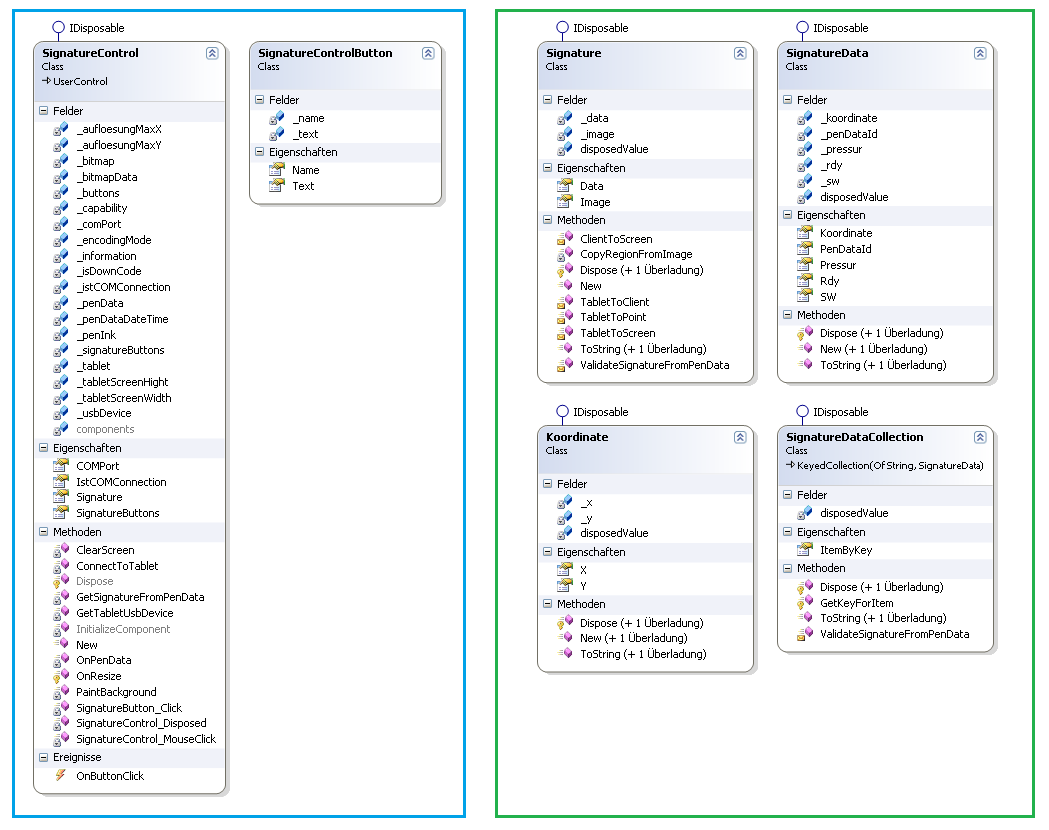
\includegraphics[height=350pt, width=\textwidth]{Klassendiagramm_FZP_Wacom_Edit1.png}
    \caption[Klassendiagramm Erstellung Steuerelement und Aufbereitung Daten]{\small{Klassendiagramm Teilprojekt Erstellung Steuerelement und Aufbereitung Daten}}
\end{figure}
\newline
\pagebreak
\textbf{} %Workaround
\newline
Die Speicherung der Daten erfolgt in der Datenbank der Sage Office Line. Die Sage Office Line benutzt eine MS SQL Datenbank. Die Abkürzung MS SQL steht für Microsoft Structured Query Language und ist ein relationales Datenbankmanagementsystem "'zum Bearbeiten (Einfügen, Verändern, Löschen) und Abfragen von darauf basierenden Datenbeständen"' \cite{sql1} \cite{sql2}. Angesichts dessen ist die Einbindung der neugeschaffenen Datenbanktabellen in das bestehende Datenbankschema problemlos zu bewerkstelligen. Die folgenden Vorteile sind maßgebend für die Nutzung von Microsoft SQL Servern. Die Verwendung von abgespeicherten Verfahrensweisen, d.h. auf einem Server wird Quellcode  gespeichert, der von Anwendungen abgefragt werden kann und zu Performanceverbesserungen von Anwendungen führt. Die Skalierbarkeit, dies bedeutet die Anpassbarkeit an das Wachstum von Unternehmen. Ein MS SQL Server ist für kleine und große Unternehmen gleichmaßen nutzbar, aufgrund der hohen Verarbeitung von Datenbankanfragen. Die Sicherheit wird mittels Benutzerkontensteuerung gewährleistet. Die Benutzerkontensteuerung regelt die Berechtigungen von einzelnen Anwendern bzw. Anwendergruppen sowie deren Eingriffsmöglichkeiten in das System. Zu den Eingriffsmöglichkeiten gehören Lese- und / oder Schreibrechte auf den Datenbanken. Ein weiterer Vorteil ist die Aufzeichnung von Datenbankabfragen, Aktualisierungen und Löschung von Datensätzen mittels Transaktionsprotokollen. Transaktionsprotokolle werden für die Systemwiederherstellung bei fehlerhaften Aktualisierungen oder Löschungen von Datensätzen verwendet. Des Weiteren besitzen MS SQL Server eine automatische Backup Funktion. Hiermit wird eine Kopie der Datenbank sowie der Transaktionsprotokolle auf weiteren Medien erstellt und somit der Schutz vor Datenverlust gesteigert. Als Nachteil von MS SQL Servern können die hohen Lizenzierungskosten sowie der exklusive Installationsort auf Microsoft Betriebssystemen genannt werden. \cite{SQLv1}